
%%%%%%%%%%%%%%%%%%%%%%%%
% $Autor: MansourAhmadyPhoulady, RanjeetsingTawar, HemanthPrabhakaran$
% $Pfad: Car_Licence_Plate_Identification_with_a_JetsonNano$
% $Version: 4.0.0 $
%
% !TeX encoding = utf8
%
%%%%%%%%%%%%%%%%%%%%%%%%

\chapter{Document Developer}
\label{chapter 8}
	
	\section{Structure and Flow}
	
\begin{itemize}
	\item \textbf{Environment Setup and Dependency Installation:} The script begins by setting up necessary directories for organizing the workflow, such as workspace, scripts, models, annotations, images, and more. It ensures that all required paths are created and that the environment is prepared for model training and evaluation.
	
	\item \textbf{Downloading Pretrained Models and Dependencies:} It proceeds to download TensorFlow models from the Model Zoo, along with installing necessary dependencies for TensorFlow Object Detection. This step is crucial for leveraging pre-existing models and their weights for transfer learning, speeding up the training process and improving model performance on specific tasks.
	
	\item \textbf{Preparing the Dataset:} The script includes steps for creating a label map and generating TFRecord files. This involves converting the dataset into a format that the TensorFlow Object Detection API can work with efficiently, enabling the model to understand the labels and the structure of the dataset.
	
	\item \textbf{Configuring the Model for Transfer Learning:} By modifying the pipeline configuration file, the script adapts a pre-trained model (SSD MobileNet V2) for the specific task, adjusting parameters such as the number of classes, batch size, and paths to training and evaluation datasets. This customization is essential for fine-tuning the model on a custom dataset.
	
	\item \textbf{Model Training and Evaluation:} Commands are provided to train the model using the prepared dataset and evaluate its performance. This phase involves iteratively adjusting the model's weights to minimize prediction errors on the training data, followed by assessing the model's accuracy on unseen data.
	
	\item \textbf{Model Export and Conversion:} The script outlines steps for exporting the trained model and converting it into TensorFlow Lite format, which is optimized for deployment on mobile devices and embedded systems. This includes instructions for freezing the model, optimizing it for inference, and converting it to a format suitable for integration into applications.
	
	\item \textbf{Utility Functions and Testing:} Additional steps include scripts for detecting objects in images using the trained model, showcasing how to utilize the model for real-world applications. This demonstrates the model's ability to identify and localize objects within images, a critical capability for many computer vision tasks.
	
	\item \textbf{Deployment Preparation:} Finally, the script hints at converting the TensorFlow Lite model into a C source file, a step towards deploying the model on hardware devices. This process involves translating the model into a format that can be directly compiled and run on microcontrollers and other low-power devices, facilitating the integration of machine learning models into IoT applications and embedded systems.
\end{itemize}
	
	\begin{center}
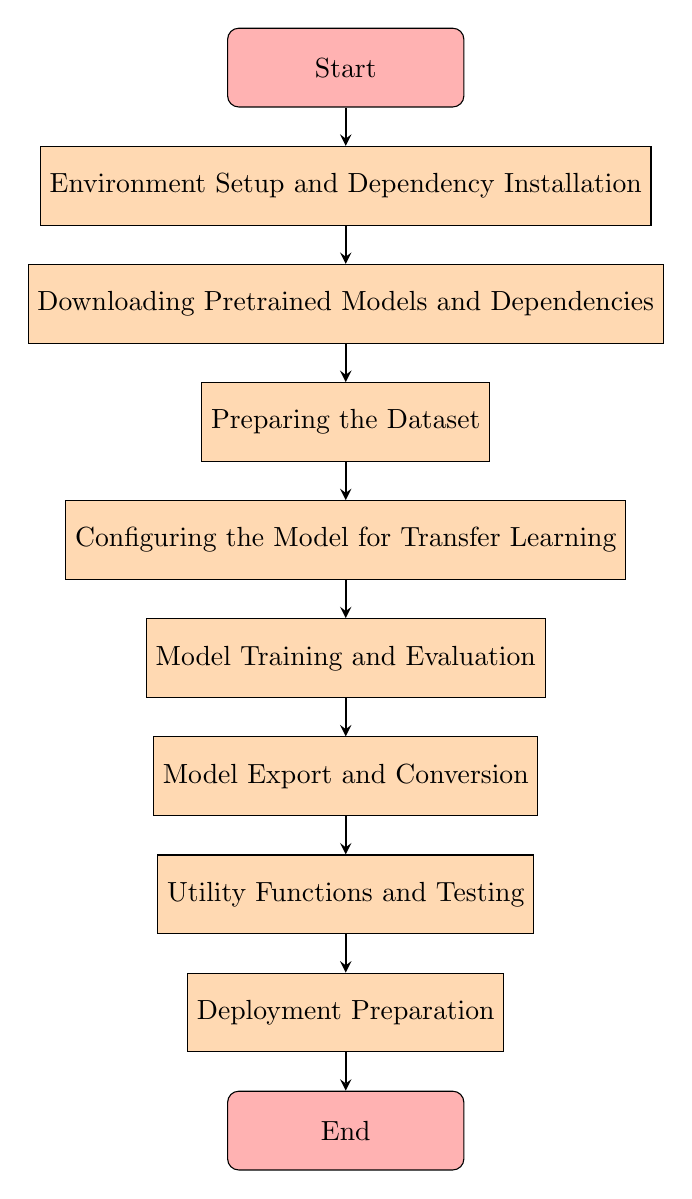
\begin{tikzpicture}[node distance=1.5cm, 
	startstop/.style={rectangle, rounded corners, minimum width=3cm, minimum height=1cm,text centered, draw=black, fill=red!30},
	process/.style={rectangle, minimum width=3cm, minimum height=1cm, text centered, draw=black, fill=orange!30},
	arrow/.style={thick,->,>=stealth}]
	
	\node (start) [startstop] {Start};
	\node (setup) [process, below of=start] {Environment Setup and Dependency Installation};
	\node (download) [process, below of=setup] {Downloading Pretrained Models and Dependencies};
	\node (prepdata) [process, below of=download] {Preparing the Dataset};
	\node (configmodel) [process, below of=prepdata] {Configuring the Model for Transfer Learning};
	\node (traineval) [process, below of=configmodel] {Model Training and Evaluation};
	\node (exportconvert) [process, below of=traineval] {Model Export and Conversion};
	\node (utiltest) [process, below of=exportconvert] {Utility Functions and Testing};
	\node (deploy) [process, below of=utiltest] {Deployment Preparation};
	\node (end) [startstop, below of=deploy] {End};
	
	\draw [arrow] (start) -- (setup);
	\draw [arrow] (setup) -- (download);
	\draw [arrow] (download) -- (prepdata);
	\draw [arrow] (prepdata) -- (configmodel);
	\draw [arrow] (configmodel) -- (traineval);
	\draw [arrow] (traineval) -- (exportconvert);
	\draw [arrow] (exportconvert) -- (utiltest);
	\draw [arrow] (utiltest) -- (deploy);
	\draw [arrow] (deploy) -- (end);
\end{tikzpicture}
	\end{center}
	

	The flowchart provides a detailed blueprint for the development of an Automated License Plate Detection System using the Jetson Nano. Beginning with the "Start" node, this outlines the project's inception. The first phase, "Environment Setup and Dependency Installation," lays the foundational work by preparing the Jetson Nano's environment and installing necessary dependencies.
	
	Progressing to "Downloading Pretrained Models and Dependencies," this step involves obtaining TensorFlow models and additional resources from the internet. This is crucial for enhancing the model's performance through transfer learning, facilitating a quicker development cycle.
	
	The journey continues with "Preparing the Dataset," focusing on gathering images of license plates and preprocessing them for training. This ensures the data is primed for the model to learn distinctive features of license plates, a critical aspect of the detection system.
	
	In "Configuring the Model for Transfer Learning," the script customizes a pre-existing model to meet the specific requirements of license plate detection. This includes adjusting parameters like the number of classes and learning rates to fine-tune the model for high precision in plate recognition.
	
	"Model Training and Evaluation" represents the pivotal phase where the tailored model is trained with the curated dataset. Its performance is rigorously evaluated to guarantee accuracy and reliability for deployment in real-world scenarios.
	
	Next, "Model Export and Conversion" transitions the trained model into a TensorFlow Lite format, suitable for deployment on the Jetson Nano. This includes quantization to compress the model size without sacrificing performance, ensuring the system's efficiency on edge devices.
	
	"Utility Functions and Testing" then tests the model's functionality with scripts designed to assess its effectiveness in identifying and recognizing license plates accurately.
	
	Finally, "Deployment Preparation" readies the system and the model for actual deployment, ensuring the Automated License Plate Detection System is set for implementation in various environments.
	
	The process concludes at the "End" node, marking the fulfillment of a methodical and comprehensive development journey. From initial setup to a deployment-ready model, the flowchart encapsulates the full spectrum of creating a robust and efficient Automated License Plate Detection System using the Jetson Nano.
	
	\section{ML Pipeline}
	
	A comprehensive Machine Learning (ML) pipeline for an \textbf{Automated License Plate Detection System} leveraging the Jetson Nano is established, encompassing a series of meticulously arranged phases for the design, training, and deployment of a machine learning model focused on detecting license plates.
	
	\section{Detailed Pipeline Phases}
	
	\begin{enumerate}
		\item \textbf{Problem Definition}:
		Objective: Detect and recognize license plates from vehicle images using the Jetson Nano.
		Input: Camera-captured images interfaced with the Jetson Nano, featuring vehicles' license plates.
		Output: Identified license plate text from the input images.
		
		\item \textbf{Data Collection}:
		Cameras connected to the Jetson Nano capture a diverse dataset of vehicle images under various conditions.
		
		\item \textbf{Data Preprocessing}:
		Normalize image data to a consistent scale and apply image augmentation to increase dataset variability.
		
		\item \textbf{Dataset Splitting}:
		Splitting the dataset into training, validation, and testing sets for comprehensive performance evaluation.
		
		\item \textbf{Model Selection and Configuration}:
		Choosing SSD MobileNet for real-time license plate detection.
		Configuring the model with:
		\begin{lstlisting}[language=Python]
			CUSTOM_MODEL_NAME = 'my_ssd_mobnet'
		\end{lstlisting}
		
		\item \textbf{Model Training}:
		Fine-tuning the pre-trained SSD MobileNet model on the license plate dataset with:
		\begin{lstlisting}[language=Python]
			!python model_main_tf2.py --model_dir=models/my_ssd_mobnet --pipeline_config_path=models/my_ssd_mobnet/pipeline.config --num_train_steps=20000
		\end{lstlisting}
		
		\item \textbf{Model Evaluation and Optimization}:
		Evaluating the model on a test dataset with:
		\begin{lstlisting}[language=Python]
			!python model_main_tf2.py --model_dir=models/my_ssd_mobnet --pipeline_config_path=models/my_ssd_mobnet/pipeline.config --checkpoint_dir=models/my_ssd_mobnet
		\end{lstlisting}
		
		\item \textbf{Model Export and Conversion}:
		Exporting the model to TensorFlow Lite format and applying quantization with:
		\begin{lstlisting}[language=Python]
			TFLITE_SCRIPT = os.path.join(paths['APIMODEL_PATH'], 'research', 'object_detection', 'export_tflite_ssd_graph.py')
		\end{lstlisting}
		
		\item \textbf{Deployment Preparation}:
		Integrating the TensorFlow Lite model into the Jetson Nano environment for real-time inference with:
		\begin{lstlisting}[language=Python]
			detect_fn = tf.saved_model.load(os.path.join(paths['OUTPUT_PATH'], 'saved_model'))
		\end{lstlisting}
		
	\end{enumerate}
	
	By following this ML pipeline, the development of the Automated License Plate Detection System is carried out systematically from data acquisition to the deployment of an efficient model on the Jetson Nano, ensuring the model's accuracy and efficiency for real-time application.


	\subsection{Why Use an ML Pipeline}
	
		\begin{enumerate}
			
			\item Structured Development: 
			
			ML pipelines provide a systematic and organized approach to model development, ensuring clarity and maintainability.
			
			\item Reproducibility: 
			
			The pipeline allows for easy reproduction of experiments, facilitating collaboration and research reproducibility.
			
			\item Hyperparameter Tuning: 
			
			Enables systematic optimization of model hyperparameters for better performance \cite{Cong:2022}.
			
			\item Ease of Debugging:
			
			A step-by-step approach makes it simpler to identify and rectify issues at each stage.
			
			\item Efficient Resource Utilization: 
			
			ML pipelines enable efficient use of computational resources by breaking down complex tasks into manageable steps.
			
			\item Scalability: 
			
			A well-defined pipeline is scalable, allowing for the incorporation of additional data and improvements without a complete overhaul.
			
			\item Deployment Readiness: 
			
			Ensures that the model is not only accurate but also optimized and ready for deployment on edge devices.
			
		\end{enumerate}
	
	An ML pipeline for the Magic Wand project streamlines the development process, enhances model performance, and ensures the successful deployment of the gesture recognition system \cite{Zhou:2020}.
	
	\subsection{Car License Plate Detection Flowchart}
	

\begin{center}
	\begin{tikzpicture}[node distance=0.5cm and 1cm, auto,
		block/.style={
			rectangle, 
			draw, 
			fill=blue!20, 
			text width=8em, 
			align=center, 
			rounded corners, 
			minimum height=4em
		},
		cloud/.style={
			draw, 
			ellipse,
			fill=green!20, 
			minimum height=1em
		},
		decision/.style={
			diamond, 
			aspect=2, 
			draw, 
			fill=yellow!20, 
			text width=7em, 
			align=center, 
			inner sep=-2pt
		},
		line/.style={
			draw, 
			-latex
		},
		every node/.style={font=\sffamily\small}
		]
		
		% Nodes
		\node [cloud] (init) {Start};
		\node [block, below=of init] (start) {Webcam is ON and\\detects for license plate};
		\node [decision, below=of start] (select) {Check if valid\\license plate};
		\node [block, left=of select, xshift=-2cm] (invalid) {Continues to\\detect again};
		\node [block, below=of select] (distance) {Rectangle Frame\\around the plate};
		\node [block, below=of distance] (update) {Text extracted\\from the plate};
		\node [block, below=of update] (run) {Check the\\threshold percentage};
		\node [decision, below=of run] (decide) {Adequate and\\accurate?};
		\node [cloud, left=of decide, xshift=-2cm] (none) {Stores nothing};
		\node [block, below=of decide, node distance=2cm] (stop) {Stores in csv\\with UUID};
		\node [cloud, below=of stop] (end) {End};
		
		% Paths
		\path [line] (init) -- (start);
		\path [line] (start) -- (select);
		\path [line] (select) -- node [near start] {yes} (distance);
		\path [line] (select) -- node [near start] {no} (invalid);
		\path [line] (invalid) |- (start);
		\path [line] (distance) -- (update);
		\path [line] (update) -- (run);
		\path [line] (run) -- (decide);
		\path [line] (decide) -- node [near start] {yes} (stop);
		\path [line] (decide) -- node [near start] {no} (none);
		\path [line] (stop) -- (end);
	\end{tikzpicture}
\end{center}
	
\noindent
The automated license plate detection process is summarized as follows:

\begin{itemize}
	\item The process \textbf{starts} with the activation of the webcam.
	\item The \textbf{webcam detects} for a license plate presence.
	\item A \textbf{decision} is made on whether a \textbf{valid license plate} is detected.
	\begin{itemize}
		\item If \textbf{no}, the system \textbf{continues to detect again}.
		\item If \textbf{yes}, a \textbf{rectangle frame} is created around the plate.
	\end{itemize}
	\item \textbf{Text is extracted} from the framed area of the plate.
	\item The system \textbf{checks the threshold percentage} of the detection accuracy.
	\begin{itemize}
		\item If the result is \textbf{not adequate and accurate}, it stores nothing and may \textbf{end} or loop back to detection.
		\item If the result is \textbf{adequate and accurate}, the information is \textbf{stored in a CSV file with a UUID}.
	\end{itemize}
	\item The process \textbf{ends} after storing the data or deciding not to store any data.
\end{itemize}
	
	
	
\begin{figure}
	\centering
	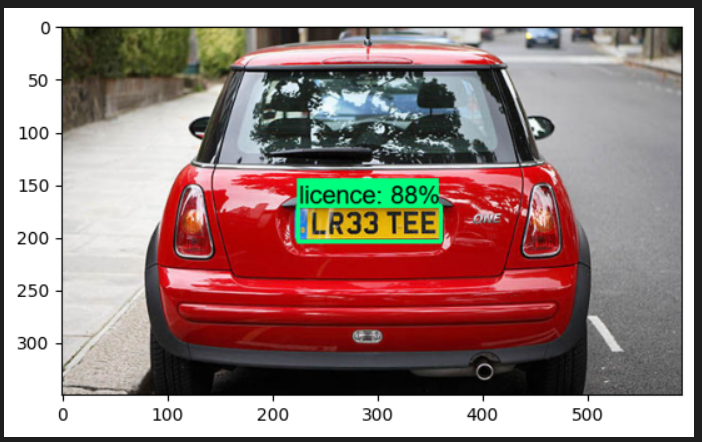
\includegraphics[width=0.7\linewidth]{Images/detection1}
	\caption{Detection of license threshold}
	\label{fig:detection1}
\end{figure}


\begin{figure}
	\centering
	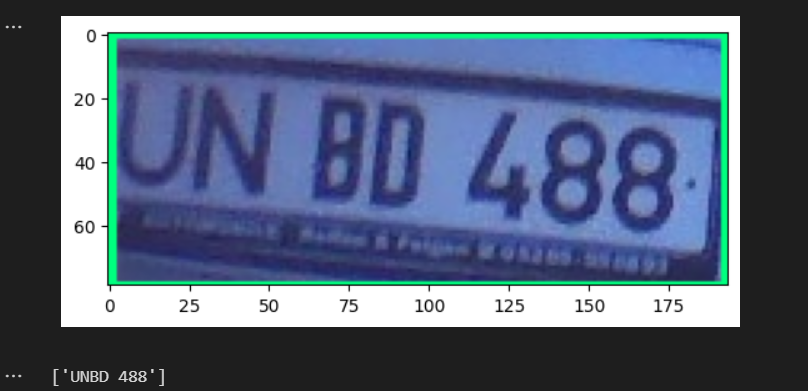
\includegraphics[width=0.7\linewidth]{Images/detection2}
	\caption{Detection of realtime number plate}
	\label{fig:detection2}
\end{figure}



\begin{figure}
	\centering
	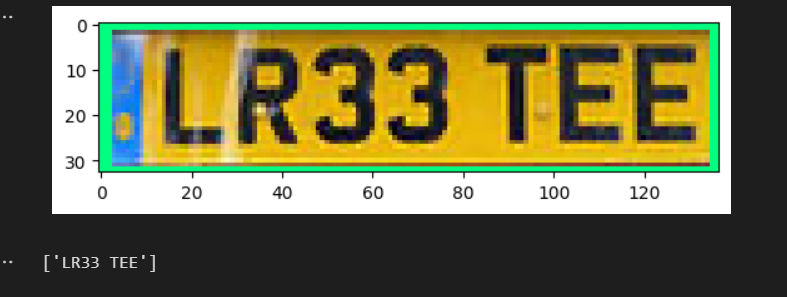
\includegraphics[width=0.7\linewidth]{Images/detection3}
	\caption{Detection of text from plate}
	\label{fig:detection3}
\end{figure}


\begin{figure}
	\centering
	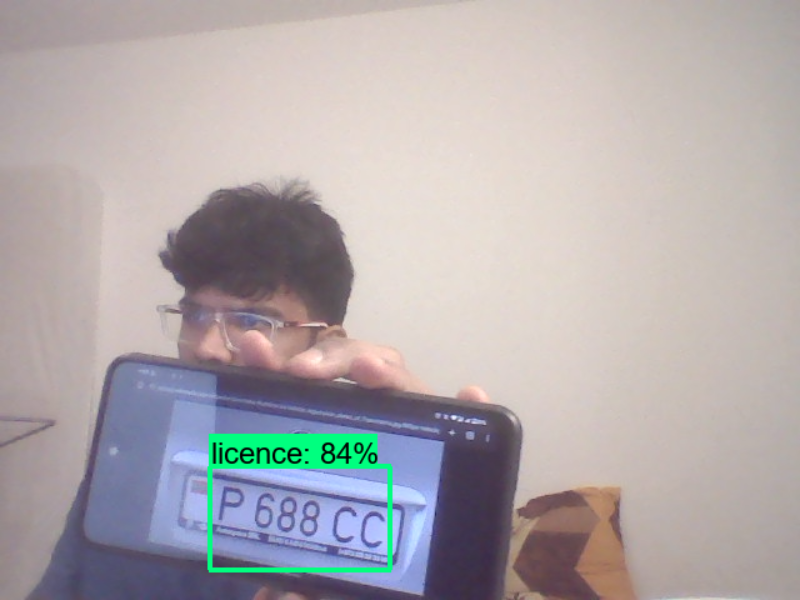
\includegraphics[width=0.7\linewidth]{Images/object_detection}
	\caption{Detection using webcam}
	\label{fig:objectdetection}
\end{figure}
